\section{Umsetzung des Lösungsweges}
\label{sec:umsetzung}

\subsection{Decodierung der STEP-Datei}

Aus dem in Abschnitt \ref{sec:eingabegeometrie} beschriebenen zeilenweisen Aufbau einer STEP-Datei lassen sich die STEP-Entitäten in Java abbilden. Jede Zeile beschreibt genau eine Entität. Diese sind stets nach dem folgenden Muster aufgebaut:

\begin{lstlisting}[captionpos=b, style=customc, caption=Beschreibung eines Punktes in STEP, label=lst:simplestp]
#ID=KLASSE(ATTRIBUTSLISTE);
\end{lstlisting}

Aufgrund dieses einheitlichen Musters lassen sie sich relativ einfach decodieren und als Java-Klassen in Programmcodes umwandeln, um in einem weiteren Schritt die Struktur des Bauteils abzubilden.
Das Ziel des ersten Schrittes in der Lösungsumsetzung besteht nun darin, aus einer einzelnen Zeile der STEP-Datei Java-Objekte zu bilden und mit den Daten aus der jeweiligen Zeile zu belegen.    

\subsubsection{Implementierte STEP-Entitäten}

Die verschiedenen Entitätstypen, die in einer STEP-Datei vorhanden sein können, sind in der STEP-Dokumentation \cite{StepDoc} aufgeführt. Die Attribute, welche zu jeder einzelnen Klasse gehören, werden darin beschrieben.
Da die Implementierung aller vorhandenen STEP-Klassen den Rahmen dieser Arbeit überschreiten würde, sind vorerst folgende Klassen im Programm umgesetzt. Es ist anzumerken, dass nicht jede Klasse eine Instanz bilden kann. Diese sogenannten abstrakten Klassen dienen der Gruppierung von ähnlichen nicht abstrakten Klassen. Diese sind Bestandteil des Vererbungsprinzips der objektorientierten Programmierung in Java. Sie sind in der Liste als solche gekennzeichnet.  
\begin{itemize}
	\item REPRESENTATION\_ITEM (abstrakt)
	\item GEOMETRIC\_REPRESENTATION\_ITEM (abstrakt)
	\item TOPOLOGICAL\_REPRESENTATION\_ITEM (abstrakt)
	\item POINT (abstrakt)
	\item CARTESIAN\_POINT
	\item DIRECTION
	\item VECTOR
	\item PLACEMENT (abstrakt)
	\item AXIS2\_PLACEMENT\_3D
	\item SURFACE (abstrakt)
	\item ELEMENTARY\_SURFACE (abstrakt)
	\item PLANE
	\item CYLINDRICAL\_SURFACE	
	\item CURVE (abstrakt)
	\item LINE
	\item CONIC (abstrakt)
	\item CIRCLE 
	\item VERTEX (abstrakt)
	\item VERTEX\_POINT
	\item EDGE (abstrakt)
	\item EDGE\_CURVE
	\item ORIENTED\_EDGE
	\item LOOP (abstrakt)
	\item EDGE\_LOOP
	\item FACE\_BOUND
	\item OUTER\_FACE\_BOUND
	\item FACE (abstrakt)
	\item FACE\_SURFACE
	\item ADVANCED\_FACE
\end{itemize}

\subsubsection{Erläuterung der implementierten STEP-Entitäten}
\label{sec:erklaerungstp}


\paragraph{CARTESIAN\_POINT}

Beschreibt einen Punkt im dreidimensionalen Raum mit den Koordinaten x, y und z (in mm), bezogen auf das Weltkoordinatensystem des in der STEP-Datei beschriebenen Bauteils. Diese Punkte dienen als Basis für viele weitere STEP-Entitäten, beziehen sich selbst aber nicht auf andere Objekte. 

\paragraph{DIRECTION}

Ebenso wie die \textit{CARTESIAN\_POINT}s beziehen sich diese Entitäten nicht auf andere. Sie repräsentieren einen normalisierten Richtungsvektor (Länge = 1 mm) mit den Richtungskoordinaten x, y, z (in mm). Diese Richtungsvektoren werden von vielen STEP-Entitäten referenziert.

\paragraph{VECTOR}

Stellt einen räumlichen Vektor dar. Dieser hat als Grundgeometrie einen normalisierten Richtungsvektor (\textit{DIRECTION}) und eine gegebene Länge. Ein \textit{VECTOR} bezieht sich demnach, anders als die vorher beschriebenen Klassen, auf ein Objekt einer anderen Klasse.

\paragraph{AXIS2\_PLACEMENT\_3D}

Beschreibt ein lokales Koordinatensystem im Raum. Es besteht aus einem \textit{CARTESIAN\_POINT}, welcher die Position des lokalen Koordinatenursprungs darstellt. Des Weiteren definieren zwei Richtungsvektoren die Ausrichtung dieses lokalen Koordinatensystems.

\paragraph{LINE}

Beschreibt eine gerade Strecke im Raum. Eine \textit{LINE} wird gebildet aus einem \textit{CARTESIAN\_POINT}, welcher den Startpunkt der Linie darstellt, sowie einem \textit{VECTOR}, welcher Richtung und Länge der Strecke bestimmt. 

\paragraph{CIRCLE}

Definiert einen Kreis im dreidimensionalen Raum. Die Position (Mittelpunkt) und Ausrichtung des Kreises wird durch ein lokales Koordinatensystem in Form eines \textit{AXIS2\_PLACE\-MENT\_3D} beschrieben. Dabei steht der erste Vektor des lokalen Koordinatensystems senkrecht auf der Ebene, in welcher der Kreis liegt. Der zweite Vektor liegt in der Kreisebene. \prettyref{fig:circleentity} verdeutlicht den Aufbau. 

\begin{figure}[h]
	\centering
	
	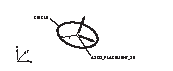
\includegraphics[width=\linewidth]{img/circle_entity.pdf}
	
	\caption{Visualisierung \textit{CIRCLE}}
	\label{fig:circleentity}
\end{figure} 

\paragraph{PLANE}

Beschreibt eine Ebene im Raum. Diese Ebene hat keine räumliche Begrenzung und ist durch einen \textit{AXIS2\_PLACEMENT\_3D} eindeutig definiert. Ähnlich wie beim \textit{CIRCLE} legt der erste Vektor des lokalen Koordinatensystems den Normalenvektor der Ebene fest. Der zweite Vektor beschreibt einen Richtungsvektor der Ebene. Durch den Koordinatenursprung des lokalen Koordinatensystems wird der Ortsvektor der Ebene definiert. 

\begin{figure}[h]
	\centering
	
	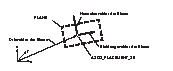
\includegraphics[width=\linewidth]{img/plane_entity.pdf}
	
	
	\caption{Visualisierung \textit{PLANE}}
	
\end{figure} 

\paragraph{CYLINDRICAL\_SURFACE}


Beschreibt analog zur \textit{PLANE} eine zylindrische Ebene im Raum. Diese kann man sich vorstellen als Mantelfläche eines unendlich langen Zylinders. Die Lage des Zylinders wird auch hier durch eine \textit{AXIS2\_PLACEMENT\_3D} definiert und hat als zusätzlichen Parameter eine Zahlenwertangabe zum Radius. In der folgenden Abbildung ist zu erkennen, dass die Achse des Zylinders aus dem ersten Vektor des lokalen Systems gebildet wird und der zweite Vektor parallel zur Deckfläche des Zylinders liegt.

\begin{figure}[h]
	\centering
	
	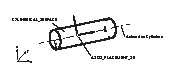
\includegraphics[width=\linewidth]{img/cylinder_entity.pdf}
	
	\caption{Visualisierung \textit{CYLINDRICAL\_SURFACE}}
	
\end{figure}

\paragraph{VERTEX\_POINT}

Definiert einen Punkt des Bauteils im Raum. Dieser wird definiert durch einen \textit{CARTESIAN\_POINT}. Der Unterschied besteht darin, dass es sich bei einem \textit{VERTEX\_POINT} um einen tatsächlichen Punkt des Bauteils (beispielsweise einen Eckpunkt einer Körperkante) handelt und nicht um eine bloße Referenz.   

\paragraph{EDGE\_CURVE}

Beschreibt eine Körperkante. Dabei kann es sich um verschiedene Kantentypen, wie Kreise, Linien oder Splines  handeln. Definiert werden Anfangs- und Endpunkt der \textit{EDGE\_CURVE}. Diese werden als Körperpunkte (VERTEX) definiert. Handelt es sich um eine geschlossene Kante, beispielsweise einen Kreis, dann sind Anfangs- und Endvertex identisch. Außerdem weist eine \textit{EDGE\_CURVE} eine Orientierung auf. Diese wird durch einen boolschen Wert (wahr oder falsch) angegeben und definiert so eindeutig Anfangs- bzw. Endpunkt der Körperkante.   

\paragraph{EDGE\_LOOP}

Beschreibt einen Kantenverbund aus mehreren Körperkanten. Dieser Kantenverbund ist geschlossen und enthält als Parameter die Liste der enthaltenen Körperkanten. 

\paragraph{FACE\_OUTER\_BOUND}

Beschreibt die äußere Umrandung einer Körperfläche und wird durch eine \textit{EDGE\_LOOP} beschrieben. Dies kann zum Beispiel ein Polygon aus verschiedenen Linien oder Kurvenstücken sein. Solch eine äußere Umrandung kann aber auch durch einen Kreis definiert sein.

\paragraph{FACE\_BOUND}

Definiert die innere Umrandung einer Körperfläche einer \textit{EDGE\_LOOP}. Dies kann, wie bei einer \textit{FACE\_OUTER\_BOUND}, ein Polygon aus verschiedenen Linien oder Kurvenstücken sein. Solch eine innere Umrandung kann aber auch durch einen Kreis definiert sein.   

\paragraph{ADVANCED\_FACE}

Beschreibt eine tatsächliche Körperfläche des in der STEP-Datei formulierten Bauteils. Definiert ist die Fläche zum einen durch eine Liste an Umrandungen (BOUNDs) zum anderen durch die Angabe einer PLANE bzw. \textit{CYLINDRICAL\_SURFACE}, in welcher diese Umrandungen liegen. Diese Körperflächen sind in ihrer räumlichen Ausdehnung begrenzt. Die Menge aller \textit{ADVANCED\_FACE}s einer STEP-Datei ergeben zusammengesetzt das beschriebene Modell des Bauteils. 

Abbildung \ref{fig:advancedfaceentity} zeigt den Aufbau einer planaren ADVANCED\_FACE aus einer äußeren Umrandung in Form eines Polygons (EDGE\_LOOP aus mehreren LINE-Entitäten) und einer inneren Umrandung durch einen Kreis.  

\begin{figure}[h]
	\centering
	
	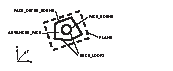
\includegraphics[width=\linewidth]{img/advancedface_entity.pdf}
	
	\caption{Visualisierung planare ADVANCED\_FACE}
	\label{fig:advancedfaceentity}
	
\end{figure}

\subsubsection{Bildung einzelner STEP-Entitäten}
\label{sec:string2entity}


Nach der Eingrenzung der zu realisierenden STEP-Entitäten und der Erklärung dieser folgt in diesem Abschnitt die Beschreibung, wie aus einer Zeile der STEP-Datei ein konkretes Java-Objekt gebildet wird. 

Zuerst müssen alle implementierten STEP-Entitäten als Java-Klassen beschrieben werden. Diese dienen als Muster für die verschiedenen Objekte der STEP-Datei. Die oben aufgeführten Klassen sind im Projektordner \textit{"`./src/main/java/com.jandoant/stp\_entities"'} zu finden. Diese enthalten die entsprechend der STEP-Dokumentation aufgeführten Attribute für jede Entität. 

In der Klasse \verb|StpEntityBuilder| im Projektordner \textit{"`./src/main/java/com.jandoant/builder"'} wird dies umgesetzt. Diese Klasse wird im Programmablauf für jede Zeile der STEP-Datei einmal aufgerufen. Übergeben wird ihr die Zeichenkette der jeweiligen Zeile. Aus dieser übergebenen Zeichenkette kann die Klasse nun mit Aufruf der Funktion \verb|extractStpEntity()| ein entsprechendes Objekt der beschriebenen STEP-Entität bilden. 
Dazu wird die beschreibende Zeichenkette in ihre drei Bestandteile (ID, Klassenname, Attributsliste) zerlegt. Über die Kenntnis des Klassennamens kann die Klasse \verb|StpEntityBuilder| entscheiden, welcher Entitätstyp erzeugt werden soll. In einem weiteren Schritt werden die Elemente der Attributsliste extrahiert und ein konkretes Java-Objekt einer STEP-Entität mit all seinen konkreten Attributen kann gebildet werden. Es ist festzustellen, dass es zu diesem Zeitpunkt noch nicht möglich ist, die tatsächlichen Referenzobjekte in der erzeugten Entität festzuhalten. Vorerst kann aus der Zeichenkette nur die jeweilige ID der Referenzobjekte gespeichert werden. Die Zuordnung kann erst erfolgen, wenn alle Zeilen der STEP-Datei in Java-Objekte ausgelesen wurden.

\subsubsection{Abbildung des gesamten STEP-Modells in Java} 

Das Programm ist, wie im vorherigen Abschnitt gezeigt, in der Lage, aus einer einzelnen Zeile der vorliegenden STEP-Datei ein konkretes Java-Objekt zu extrahieren. Nun folgt in diesem Schritt die Decodierung der gesamten Datei. Nach Beendigung dieses Vorgangs ist die komplette geometrische Bauteilstruktur im Programm abgebildet und kann darauffolgend weiter verarbeitet werden.

Der Vorgang dieser Decodierung erfolgt durch die Klasse \verb|StpModelBuilder|, welche sich im Projektordner \textit{"`./src/main/java/com.jandoant/builder"'} befindet. 
Wird diese Klasse im Pro\-gramm\-ab\-lauf instanziiert, so wird ihr der absolute Pfad, unter dem die zu verarbeitende STEP-Datei liegt, übergeben. Mit dieser Information hat die erzeuge Instanz den Zugriff auf alle Zeilen der Datei, welche die Bauteilgeometrie beschreiben.
Mit Aufruf der Funktion \verb|parseFile()| wird die übergebene STEP-Datei verarbeitet. Dabei werden zunächst alle Zeilen der Datei durchlaufen. Jede Zeichenkette, die eine STEP-Entität beschreibt, also mit dem \#-Symbol beginnt und mit einem Semikolon endet, wird in einer Liste dieser Zeichenketten zwischengespeichert. Es ist dabei unerheblich, ob die Zeichenkette durch einen oder mehrere Zeilenumbrüche getrennt ist. Dies hat den Effekt, dass die HEADER-Sektion herausgefiltert wird. Diese hat keine Bedeutung für die grundlegende Funktion des Programms, da in diesem Abschnitt der Datei keine STEP-Entitäten beschrieben werden.

Aus der erzeugten Liste an Zeichenketten, welche dem gewünschten Muster entsprechen, werden im folgenden Bearbeitungsschritt unter Anwendung der in \prettyref{sec:string2entity} dargelegten Methode \verb|extractStpEntity| der Klasse  \verb|StpEntityBuilder| die jeweilig beschriebenen STEP-Entitäten im Java-Code instanziiert und in einer Liste zwischengespeichert. Dabei ist anzumerken, dass ausschließlich die in der Klasse \verb|StpEntityContract| im Projektordner \textit{"`./src/\-main/\-java/\-com.jandoant/\-stp\_entities"'} festgehaltenen STEP-Entitäten decodiert werden. Alle Zeichenketten, die nicht eine solche Entität beschreiben, werden ignoriert. Das führt dazu, dass ausschließlich die geometrischen Informationen des Modells extrahiert werden. Andere Angaben, die in der STEP-Datei festgehalten sein können, werden bei dieser Implementierung nicht berücksichtigt, da sie für die grundlegende Funktion des Programmes unerheblich sind.

Nach dem Durchlaufen aller Zeilen und anschließender Instanziierung der Java-Objekte entsprechend der STEP-Beschreibung liegt zu diesem Punkt eine Liste mit allen vorkommenden geometrischen STEP-Entitäten im Programm vor. Allerdings ist damit den Anforderungen noch nicht entsprochen. Nach der Decodierung der einzelnen Zeichenketten haben die Java-Objekte noch keine Relation zueinander. Wie in \prettyref{sec:string2entity} erläutert, sind die Referenzentitäten, auf die sich eine STEP-Entität bezieht, bisher nur mit ihrer ID erfasst. Eine Zuordnung der Objekte passiert nun aus vorliegender Liste der erzeugten Java-Objekte. 
Dazu wird die Methode \verb|convertFromIds()| aufgerufen, welche in jeder Java-Klasse, die eine STEP-Entität beschreibt, implementiert ist.
Mit Aufruf der Methode durch das betreffende Java-Objekt wird die Entitätsliste durchlaufen. Dabei werden alle Entitäten, deren ID mit einer der IDs, die in diesem Java-Objekt hinterlegt sind, herausgefiltert und dem Java-Objekt zugewiesen. Nachdem dieser Vorgang für alle Objekte der Liste ausgeführt wurde, sind alle Referenzen über tatsächliche Java-Objekte hergestellt. 

Die im Programmablauf aufgerufene Methode \verb|parseFile()| der Klasse \verb|StpModelBuilder| gibt nun in einem finalen Schritt alle \textit{ADVANCED\_FACE}s, die in der STEP-Datei durch Zeichenketten beschrieben wurden, als tatsächliche Java-Objekte an das Programm zurück. Dies geschieht in Form einer Liste. Diese \textit{ADVANCED\_FACE}s  referenzieren wie oben beschrieben alle Objekte, durch welche sie selbst definiert werden. Somit ist die gesamte Bauteilstruktur im Programm abgebildet und kann im weiteren Ablauf des Programms verarbeitet werden.

\subsection{Diskretisierung der Körperflächen}

Die Diskretisierung der Oberflächen wird unter Einführung eines lokalen Koordinatensystems für jede einzelne Körperfläche (\textit{ADVANCED\_FACE}) realisiert.
Ziel ist dabei die Umwandlung der Punkte der Körperflächen, welche durch die STEP-Datei in globalen Koordinaten ausgedrückt sind, in ein lokales Koordinatensystem zu überführen und im Anschluss zu verändern. Dabei werden alle Punkte der jeweiligen Fläche einer Koordinatentransformation unterzogen. So besitzt jeder Punkt neben seiner Beschreibung im Weltkoordinatensystem mit Werten in x-, y- und z-Richtung gleichzeitig auch Definitionen bezüglich eines lokalen Koordinatensystems in u-, v- und w-Richtung. Die folgende \prettyref{fig:basetrafo} verdeutlicht dies. 

\begin{figure}[h]
	\centering
	
	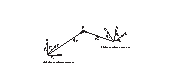
\includegraphics[width=\linewidth]{img/basetrafo.pdf}
	
	\caption{Beschreibung eines Punktes in verschiedenen Koordinatensystemen}
	\label{fig:basetrafo}
	
\end{figure}

Das lokale Koordinatensystem ist spezifisch für jede Körperfläche und ermöglicht eine generalisierte Bearbeitung der diskretisierten Punkte. Jede dreidimensionale Körperfläche wird so in eine zweidimensionale Fläche mit Ausdehnung in u- und v-Richtung überführt. Die w-Koordinate, welche senkrecht zur Fläche zeigt, ist dabei für die Idealgeometrie w = 0. Dieses Verfahren wird als "`UV-Mapping"' bezeichnet. Mit der Anwendung der Deformationsfunktionen ändert sich die Koordinate der Punkte in dieser Richtung. Eine Rücktransformation in das globale Koordinatensystem bildet diese Veränderung an der deformierten Geometrie ab.       

\begin{figure}[h]
	\centering
	
	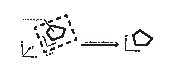
\includegraphics[width=\linewidth]{img/uvwmapping.pdf}
	
	\caption{UV-Mapping einer Körperfläche}
	\label{fig:uvwmapping}
	
\end{figure}
 
\subsubsection{Basistransformation}
\label{sec:basetransform}


Um eine Basistransformation zwischen Welt- und lokalem Koordinatensystem durchführen zu können, ist es notwendig, sowohl die Basiseinheitsvektoren des Weltkoordinatensystems als auch die des lokalen Systems zu kennen. Die Basiseinheitsvektoren des globalen Koordinatensystems sind für alle Punkte des STEP-Modells stets dieselben und werden wie folgt definiert.

\begin{singlespace}
	\begin{equation}
	\begin{aligned}
	\vv{e_{x}}=\begin{pmatrix}
	1 \\ 
	0 \\ 
	0
	\end{pmatrix}  
	&& 
	\vv{e_{y}}=\begin{pmatrix}
	0 \\ 
	1 \\ 
	0
	\end{pmatrix}  
	&& 
	\vv{e_{z}}=\begin{pmatrix}
	0 \\ 
	0 \\ 
	1
	\end{pmatrix} 
	\end{aligned}
	\end{equation}
\end{singlespace}

Die Menge aller Punkte einer Ebene wird in der Geometrie durch die Formel

\begin{equation}\label{eq:plane}
E: \vv{x} = \vv{x_{0}} + r \cdot \vv{x_{R1}} + s \cdot \vv{x_{R2}}  
\end{equation}

eindeutig festgelegt. Dabei steht $\vv{x}$ für einen beliebigen Punkt der Ebene. $\vv{x_{0}}$ beschreibt den Ortsvektor, $\vv{x_{R1}}$ und $\vv{x_{R2}}$  die Richtungsvektoren und $r$ und $s$ sind beliebige Laufparameter, um die Lage des Punktes als Linearkombination der Richtungsvektoren genau zu beschreiben.

Die Position einer \textit{PLANE} wird durch eine \textit{AXIS2\_PLACEMENT\_3D} beschrieben. Daraus lassen sich die Elemente einer Ebenenbeschreibung, wie in \prettyref{eq:plane} dargestellt, auslesen. 
Dabei entspricht der \textit{CARTESIAN\_POINT} der Positionsbeschreibung dem Ortsvektor. Dieser stellt gleichzeitig den Koordinatenursprung des lokalen Koordinatensystems dar. Die erste \textit{DIRECTION} dieser Positionsbeschreibung entspricht dem normalisierten Normalenvektor der Ebene $\vv{n}$, die zweite \textit{DIRECTION} einem normalisierten Richtungsvektor $\vv{x_{R1}}$. Da in der Lagebeschreibung der Ebene nur der Normalenvektor und ein Richtungsvektor dieser Ebene beschrieben sind, wird der fehlende Richtungsvektor durch Bildung des Kreuzproduktes der beiden für ein rechtshändiges System nach \prettyref{eq:crossproduct} erzeugt.

\begin{equation}\label{eq:crossproduct}
\vv{x_{R2}} = \vv{n} \times \vv{x_{R1}}
\end{equation}  

Ebenso, wie bei einer ebenen Fläche, die durch die STEP-Entität \textit{PLANE} beschrieben wird, wird auch bei zylindrischen Flächen des Typs \textit{CYLINDRICAL\_SURFACE} die Ausrichtung des lokalen Koordinatensystems in einem \textit{AXIS2\_PLACEMENT\_3D} festgehalten. Dabei unterscheidet sich allerdings die Bedeutung der \textit{DIRECTION}s der Positionsbeschreibung. Der \textit{CARTESIAN\_POINT} des \textit{AXIS2\_PLACEMENT\_3D} beschreibt dabei die Position des Ortsvektors der Fläche, die erste \textit{DIRECTION} die Richtung der Achse $\vv{n}$ des Zylinders und die zweite \textit{DIRECTION} $\vv{x_{R1}}$ liegt parallel zur radialen Richtung des Zylinders. Mit Hilfe der \prettyref{eq:crossproduct} lässt sich auch hier ein weiterer Vektor bilden, welcher rechtshändig orientiert senkrecht zur Achse und $\vv{x_{R1}}$ ebenfalls in radiale Richtung des Zylinder zeigt. 

Die lokalen Basiseinheitsvektoren \begin{singlespace} $\vv{e_{u}}=\begin{pmatrix}
	e_{u_x} & e_{u_y} & e_{u_z}
	\end{pmatrix}^T $, 
	$\vv{e_{v}}=\begin{pmatrix}
	e_{u_x} & e_{u_y} & e_{u_z}
	\end{pmatrix}^T$ und 
	$\vv{e_{w}}=\begin{pmatrix}
	e_{u_x} & e_{u_y} & e_{u_z}
	\end{pmatrix}^T$ 
\end{singlespace} können somit entsprechend \prettyref{eq:basevectorsuvw}  gebildet werden. Darüber wird definiert, in welche Richtung u-, v- und w-Koordinaten jeweils zeigen. 

\begin{equation}\label{eq:basevectorsuvw}
	\begin{aligned}
	\vv{e_{u}}=\vv{x_{R1}} 
	&& 
	\vv{e_{v}}=\vv{x_{R2}}  
	&& 
	\vv{e_{w}}=\vv{n} 
	\end{aligned}
\end{equation}

Sind die Basiseinheitsvektoren der beiden Koordinatensysteme bekannt, so lassen sich die jeweiligen Basismatrizen  durch spaltenweise Aneinanderreihung der Vektoren bilden. Die Basis des Weltkoordinatensystems ergibt sich damit zur Basismatrix $B_{XYZ}$ nach \prettyref{eq:basematrixxyz}. 

\begin{singlespace}
	\begin{equation}\label{eq:basematrixxyz}
		B_{XYZ} = \begin{pmatrix}
		1 & 0 & 0 \\ 
		0 & 1 & 0 \\ 
		0 & 0 & 1
		\end{pmatrix} 
	\end{equation} 
\end{singlespace}

Die Basis des Weltkoordinatensystems ergibt sich analog zur Basismatrix $B_{UVW}$ nach \prettyref{eq:basematrixuvw}.

\begin{singlespace}
	\begin{equation}\label{eq:basematrixuvw}
	B_{UVW} = \begin{pmatrix}
	e_{u_x} & e_{v_x} & e_{w_x} \\ 
	e_{u_y} & e_{v_y} & e_{w_y} \\ 
	e_{u_z} & e_{v_z} & e_{w_z}
	\end{pmatrix} 
	\end{equation} 
\end{singlespace}

Die Transformationsmatrix, um einen Punkt vom globalen in das lokale Koordinatensystem der Ebene zu transformieren, ergibt sich nach \prettyref{eq:matrixXYZ2UVW}.

\begin{equation}\label{eq:matrixXYZ2UVW}
T_{xyz \rightarrow uvw} = B_{uvw}^{-1} \cdot B_{xyz}  
\end{equation}   

Die Transformationsmatrix, um einen Punkt wieder aus dem lokalen Koordinatensystem der Ebene zurück in das globale System zu überführen, ergibt sich nach \prettyref{eq:matrixUVW2XYZ} aus der Inversen der in \prettyref{eq:matrixXYZ2UVW} berechneten Transformationsmatrix.

\begin{equation}\label{eq:matrixUVW2XYZ}
T_{uvw \rightarrow xyz} = T_{xyz \rightarrow uvw}^{-1} 
\end{equation}   

Hat man einen Punkt $\vv{p_{xyz}}$ in globale Koordinaten gegeben, so berechnet sich seine Position im lokalen Koordinatensystem entsprechend \prettyref{eq:trafoxyz2uvw}. 

\begin{equation}\label{eq:trafoxyz2uvw}
\vv{p_{uvw}}=T_{xyz \rightarrow uvw} \cdot \vv{p_{xyz}}
\end{equation}

Analog dazu berechnet man die Rücktransformation eines Punktes $\vv{p_{uvw}}$ vom lokalen Koordinatensystem in das globale Koordinatensystem nach \prettyref{eq:trafouvw2xyz}.
  
\begin{equation}\label{eq:trafouvw2xyz}
\vv{p_{xyz}}=T_{uvw \rightarrow xyz} \cdot \vv{p_{uvw}}
\end{equation}

Die Berechnung einer speziellen Transformationsmatrix ist in den Klassen \verb|StpPlane|, für planare Ebenen sowie \verb|StpCylindricalFace|, für zylindrische Oberflächen implementiert.  Diese befinden sich im Projektordner \textit{"`./src/main/java/com.jandoant/stp\_entities"'}.\\ 
Die Methode \verb|getXYZtoUVWTransformationMatrix()| ermittelt die Transformationsmatrix für die Umwandlung eines Punktes in lokale Koordinaten. Die Matrix zur Rücktransformation wird über die Methode \verb|getUVWtoXYZTransformationMatrix()| berechnet. 
Die Anwendung dieser Matrizen erfolgt in der Klasse \verb|StpCartesianPoint| im selben Projektordner.\\ 
Die Methode \verb|baseTransform(Matrix transformationMatrix)| nimmt eine Transformationsmatrix entgegen und gibt einen entsprechend der Formeln \ref{eq:trafoxyz2uvw} bzw. \ref{eq:trafouvw2xyz} transformierten Punkt aus. 

\subsubsection{Diskretisierung zylindrischer Flächen}

Zylindrische \textit{ADVANCED\_FACE}s werden in einer STEP-Datei durch eine \textit{CYLINDRICAL\_SURFACE} und zwei\textit{CIRCLE}s definiert. Dabei entspricht die \textit{CYLINDRICAL\_SURFACE}, wie in \prettyref{sec:erklaerungstp} bereits erläutert, der Mantelfläche des Zylinders. Die Begrenzungen des Zylinders ergeben sich aus der Lage der beiden Kreise (STEP-Entität \textit{CIRCLE}), die als \textit{FACE\_\-OUTER\_\-BOUND}s in der STEP-Datei formuliert sind. Der Abstand der beiden Kreise ergibt somit die gesamte Länge der zylindrischen Körperfläche.

Um eine zylindrische \textit{ADVANCED\_FACE} zu diskretisieren, müssen die Positionen der \textit{CYLINDRICAL\_SURFACE} und der \textit{CIRCLE}s, gegeben durch jeweils ein \textit{AXIS2\_PLACEMENT\_3D}, gefunden werden. Im Anschluss werden diese Positionen aus dem globalen in ein lokales Koordinatensystem transformiert. Dies ermöglicht einen generalisierten Diskretisierungsvorgang für Zylinder, unabhängig von ihrer Lage im Raum. Die Transformationsmatrix für eine \textit{CYLINDRICAL\_SURFACE} ergibt sich, wie im vorherigen Abschnitt \ref{sec:basetransform} beschrieben.  

\begin{figure}[h]
	\centering
	
	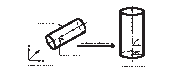
\includegraphics[width=\linewidth]{img/trafozylinder.pdf}
	
	\caption{Koordinatentransformation CYLINDRICAL\_SURFACE}
	\label{fig:trafozylinder}
	
\end{figure}

Die Abwicklung der zylindrischen Mantelfläche ergibt ein Rechteck. Dieses entspricht in seiner Breite dem Umfang des Kreisprofils des Zylinders und in der Höhe der Länge des Zylinders. Eine Rechteckfläche ist sehr einfach durch ein gleichmäßiges Punkteraster zu diskretisieren. Dabei ist es notwendig, zuerst die Abwicklung durchzuführen. Über die Transformation der lokalen kartesischen Koordinaten in u-, v- und w-Richtung in lokale zylindrische Koordinaten soll dies umgesetzt werden. Nach erfolgter Transformation in das zylindrische Koordinatensystem kann jeder Punkt auf der Zylinderoberfläche als Punkt auf der abgewickelten Mantelfläche in zylindrischen Koordinaten ausgedrückt werden. \prettyref{fig:discretzylinder} soll den Sachverhalt darstellen. 

\begin{figure}[h]
	\centering
	
	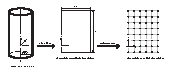
\includegraphics[width=\linewidth]{img/discretzylinder.pdf}
	
	\caption{Abwicklung und Diskretisierung einer zylindrischen Körperfläche}
	\label{fig:discretzylinder}
	
\end{figure}

Die Transformation eines kartesischen Punktes der Zylinderoberfläche kann mit den folgenden Formeln in einen Punkt in zylindrischen Koordinaten umgerechnet werden.
Wenn gilt 
\begin{singlespace}
 \begin{equation}
 	\begin{aligned}
	 	\vv{p_{uvw}} = \begin{pmatrix}
	 	u & v & w
	 	\end{pmatrix}^T \\
	 	\vv{p_{r\varphi w}} = \begin{pmatrix}
	 	\varphi & w & r
	 	\end{pmatrix}^T	 	 	
	 \end{aligned}
 \end{equation}
\end{singlespace}
dann ergeben sich die zylindrischen Koordinaten bei gegebenen kartesischen Koordinaten nach
\begin{equation}	
	\begin{aligned}
		r &= \sqrt{u^2 + v^2} \\
		\varphi &= {\arctan{\frac{v}{u}}}
	\end{aligned}	
\end{equation}
Der Wert in w-Richtung ändert sich dabei nicht.

Analog dazu lässt sich auch die Rücktransformation in kartesische Koordinaten bei gegebenen zylindrischen Koordinaten durchführen. Auch dabei ändert sich die w-Koordinate nicht.
\begin{equation}\label{eq:cyl2uvw}	
	\begin{aligned}
		u &= r \cdot \cos{\varphi}  \\
		v &= r \cdot \sin{\varphi}
	\end{aligned}	
\end{equation}

Um die Diskretisierung einer gegebenen zylindrischen \textit{ADVANCED\_FACE} durchzuführen, ist es also notwendig, diese abgewickelte Rechteckfläche mit einem Punkteraster zu versehen. Der Nutzer kann dabei angeben, in wieviele axiale Ringe und wieviele Zylindersegmente die Fläche zerlegt werden soll. Aufgrund dieser Angaben wird das Punkteraster entsprechend erstellt. Das Programm berechnet aus der gewünschten Anzahl der Ringe die Abstände in w-Richtung, aus der Angabe der Anzahl der Zylindersegmente den Abstand in $\varphi$-Richtung. Beginnend bei der w-Koordinate des Mittelpunkts des ersten \textit{CIRCLE}s und der Winkelkoordinate $\varphi = 0$ wird das Raster bis zur w-Koordinate des zweiten \textit{CIRCLE}s und $\varphi = 2\pi$ in den benötigten Abständen aufgezogen. Jeder erzeugte Punkt des Rasters wird in der Punktewolke der \textit{ADVANCED\_FACE} gespeichert und kann bei Deformation der Fläche verändert werden. 

\subsubsection{Diskretisierung planarer Flächen}
\label{sec:discreteplanar}

Planare \textit{ADVANCED\_FACE}s werden in STEP durch die \textit{PLANE}, auf der sie liegen, und einer bestimmten Anzahl an Umrandungen beschrieben. Die Menge aller Punkte, die zu dieser \textit{ADVANCED\_FACE} gehören, ergibt sich aus der Schnittmenge aller Punkte der PLANE und den Punkten innerhalb der positiven Umrandungen (\textit{FACE\_OUTER\_BOUND}s) ohne die Punkte, die innerhalb der negativen Umrandung liegen. 
Dies ist durch folgende Abbildung zu visualisieren.

\begin{figure}[h]
	\centering
	
	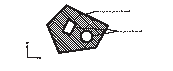
\includegraphics[width=\linewidth]{img/posnegbounds.pdf}
	
	\caption{Planare \textit{ADVANCED\_FACE} mit negativen Umrandungen}
	\label{fig:posnegbounds}
	
\end{figure}

Bei der Diskretisierung planarer Flächen wird unterschieden zwischen kreisförmigen Umrandungen und Umrandungen, die aus einem Polygon bestehen.

Als erstes soll die Diskretisierung von positiven kreisförmigen Umrandungen beschrieben werden. Dazu wird die kreisförmige Fläche in Ringe und Segmente unterteilt. Der Nutzer kann für jede Umrandung die Anzahl dieser angeben und somit die Detaillierung der Diskretisierung steuern. Die Schnittpunkte dieser Elemente sollen als Objekte der Klasse \verb|StpCartesianPoint| in der Punktewolke der Körperfläche gespeichert werden. 

\begin{figure}[h]
	\centering
	
	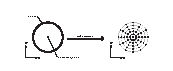
\includegraphics[width=\linewidth]{img/discretcircle.pdf}
	
	\caption{Diskretisierungsmuster Kreis}
	\label{fig:discretecircle}
	
\end{figure}

Wie in \prettyref{sec:erklaerungstp} beschrieben, besteht eine einzelne Umrandung einer \textit{ADVANCED\_FACE} aus einem Kantenverbund (\textit{EDGE\_LOOP}). Bei kreisförmigen Umrandungen wird dieser Kantenverbund genau aus einer Kante des Typs \textit{CIRCLE} gebildet. Diese Entität enthält Informationen zur Position des Kreises (in Form einer \textit{AXIS2\_PLACEMENT\_3D}) und dessen Radius.
Mit dieser Kenntnis kann die Lage des Kreises, bezogen auf das lokale Koordinatensystem, bestimmt werden. Dazu muss auch der Mittelpunkt des Kreises in das lokale Koordinatensystem transformiert werden. Ausgehend vom Radius des zu diskretisierenden Kreises und der Angabe der Anzahl an geforderten Ringen, errechnet das Programm den radialen Abstand der Ringe zueinander. Aus der Anzahl der geforderten Segmente sind in gleicher Weise auch die Öffnungswinkel der Segmente bekannt. Um nun die diskretisierte Punktemenge der Kreisfläche zu erzeugen, wird ein Startpunkt gewählt, welcher auf dem Kreis liegt. Dieser wird um den Mittelpunkt des Kreises und den Öffnungswinkel der Kreissegmente gedreht. Seine neue Position wird in der Punktewolke der betreffenden \textit{ADVANCED\_FACE} gespeichert. Danach wird dieser Vorgang wiederholt, bis die Summe der überstrichenen Öffnungswinkel 360° beträgt. Als Ergebnis dieses Vorgangs entsteht nun ein diskretisierter Ring mit dem Radius des Kreises. Nach Bildung des ersten Ringes wird ein neuer Startpunkt gewählt und von diesem aus analog ein weiterer Ring erzeugt. Dieser Vorgang wird so oft wiederholt, bis die geforderte Anzahl an Ringen hergestellt ist. 

Die Diskretisierung positiver polygonaler Umrandungen geschieht ein wenig anders. Dabei sollen sowohl die Kanten als auch der Innenraum des Polygons entsprechend \prettyref{fig:discretpolygon} in einem vom Nutzer wählbaren Abstand der Punkte  diskretisiert werden. Dazu sollen in einem ersten Schritt alle Kanten des Polygons im vorgegebenen Abstand unterteilt werden. Danach soll ein Punkteraster mit Punkten dieses Abstandes über das Innere des Polygons gelegt werden. Dazu ist es notwendig, alle Eckpunkte, die das Polygon besitzt, zu finden. Das geschieht über den Kantenverbund der (\textit{EDGE\_LOOP}) Umrandung. Dieser ist, anders als bei kreisförmigen Umrandungen, aus mindestens 3 Kanten aufgebaut. Diese Kanten sind vom Typ \textit{LINE}. Aus der einzelnen Kante lassen sich sowohl Anfangs- als auch Endpunkt der \textit{LINE} auslesen. Somit lassen sich die Eckpunkte des Polygons extrahieren. Nachdem die Menge der Eckpunkte des Polygons ermittelt wurde, werden alle diese Punkte in das lokale Koordinatensystem der Ebene unter Anwendung der Transformationsmatrix umgerechnet.
Aus der Kenntnis der Eckpunkte kann nun ein Punkt entlang der Kanten im vorgegebenen Abstand bewegt werden. Nach jedem Einzelschritt wird der Punkt der Punktewolke der \textit{ADVANCED\_FACE} hinzugefügt. 
Um das Innere des Polygons zu diskretisieren, muss zunächst das umgrenzende Rechteck gefunden werden. Innerhalb der Grenzen dieses Rechtecks wird ein Punkteraster im vorgegebenen Abstand erzeugt. Für jeden Punkt wird individuell entschieden, ob er inner- oder außerhalb des Polygons liegt. Liegt ein Punkt dieses Rasters innerhalb des Polygons, dann wird er zur Punktewolke der Körperfläche hinzugefügt.  

\begin{figure}[h]
	\centering
	
	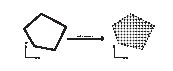
\includegraphics[width=\linewidth]{img/discretpolygon.pdf}
	
	\caption{Diskretisierungsmuster Polygon}
	\label{fig:discretpolygon}
	
\end{figure}

Alle Punkte, die innerhalb einer negativen Umrandung (kreisförmig oder polygonal) liegen, sollen aus der bestehenden Punktewolke der betreffenden \textit{ADVANCED\_FACE} entfernt werden. Dazu wird für jeden bestehenden Punkt geprüft, ob dies der Fall ist. Um allerdings die Kanten negativer Umrandungen in der Punktewolke zu behalten, werden diese entsprechend der Parameter unterteilt und der Punktwolke hinzugefügt.

\subsection{Deformation der Körperflächen}

Die Deformation der einzelnen Punkte einer Körperfläche wird über die Anwendung dreidimensionaler Funktionen realisiert. Die Punkt liegen zu diesem Zeitpunkt des Programmablaufs in lokalen Koordinaten vor. Dabei haben Punkte, die auf einer \textit{PLANE} liegen Koordinaten in u-, v- und w-Richtung. Bei diesen werden die Werte in w-Richtung durch die jeweilige Deformationsfunktion der Form $w = w_0 + f(u,v)$ verändert. Punkte, welche auf einer \textit{CYLINDRICAL\_SURFACE} liegen haben hingegen lokale Koordianten in $\varphi$-, w- und r-Richtung. Die R-Koordinate wird dabei durch eine Deformationsfunktion der Form $r=r_0+f(\varphi, w)$ berechnet. Die Werte $w_0$ bzw. $r_0$ stellen dabei den Wert der jeweiligen Koordinate vor Anwendung der Deformation dar.
Es können für jede Körperfläche unterschiedlich viele Deformationen beaufschlagt werden. Dies führt zu einer Kumulation der Verschiebungen. Damit kann man unterschiedliche Oberflächenabweichungen überlagern.
Die verschiedenen Deformationsfunktionen sind im Quellcode unter dem Projektordner \textit{"`./src/\-main/\-java/\-com.jandoant/deformation"'} zu finden. Jede Klasse in diesem Ordner stellt jeweils eine Deformationsfunktion dar. Diese implementieren alle das Interface \verb|DeformationFunction| im selben Ordner. Das dient dazu, dass alle Deformationsfunktionen der oben beschriebenen Form entsprechen und der Funktionswerts stets von zwei Variablen abhängig ist. Zur Anwendung kommt eine Deformationsfunktion durch den Aufruf der Methode \verb|applyDeformationFunction(DeformationFunction df)| der Klasse \verb|StpAdvancedFace| im Ordner \textit{"`./src/\-main/\-java/\-com.jandoant/stp\_entites"'}. Durch die Anwendung der Funktion addieren sich die dritte Koordinate des jeweiligen Punktes und der Funktionswert der Deformationsfunktion an der Stelle des Punktes. So wird die w- bzw. $\varphi$-Koordinate des durch die Deformation verschobenen Punktes gebildet. Im Programm sind ein paar beispielhafte Funktionen definiert. Aufgabe einer Weiterentwicklung des Programms besteht in der Erweiterung und Optimierung dieses Angebotes an Deformationsfunktionen um Oberflächenabweichungen realistisch abbilden zu können.

Im Folgenden sollen die bereits implementierten Funktionen kurz vorgestellt werden. Dabei werden die Funktionen zur Veränderung planarer Flächen dargestellt. Diese lassen sich aber ebenfalls für zylindrische Flächen anwenden, wenn man u- und v-Koordinate jeweils durch $\varphi$ und w-Koordinate des Zylinders ersetzt. 

\paragraph{Konstanter Faktor} Auf die Fläche wird ein konstantes Offset aufgegeben. Bei ebenen Flächen führt dies zu einer Absenkung oder Anhebung der Fläche in Normalenrichtung der Ebene. Bei Zylindrischen Flächen führt die Anwendung zu einer Erhöhung oder Verringerung des Radius. 
Die Funktion folgt der folgenden Vorschrift. Sie ist implementiert in der Klasse \verb|DeformConstant| und erhält als Parameter den zu verwendenden konstanten Wert. 
\begin{equation}\label{eq:constant}
	f(u,v) = \mathrm{c_0}
\end{equation}

\paragraph{Linear in einer Richtung} Wird auf eine ebene Fläche diese Funktion aufgegeben, dann bildet sich eine schiefe Ebene in der angegebenen Richtung. Bei der Anwendung der Funktion auf zylindrische Flächen ergibt nur die Anwendung in axialer Richtung Sinn. So kann bei zylindrischen Flächen eine konische Form hergestellt werden. Die Funktion folgt der folgenden Vorschrift und erhält als Parameter den Anstieg $\mathrm{c_1}$, die Verschiebung $\mathrm{c_0}$ der Punkte senkrecht zur Ebene bzw. Achse und die Richtung der Neigung. 

\begin{equation}	
	\begin{aligned}\label{eq:linear}
		f(u,v) = \mathrm{a_1}\cdot u+\mathrm{c_0}&&\mathrm{bzw.}&&f(u,v) = \mathrm{a_1}\cdot v+\mathrm{c_0}
	\end{aligned}
\end{equation}

Abbildung XYZ stellt die Funktion grafisch dar. Implementiert ist die Funktion in der Klasse \verb|DeformLinear|.

\paragraph{Linear in zwei Richtungen} Ähnlich wie bei der vorher beschriebenen Funktion erzeugt diese Deformation eine schiefe Ebene. Allerdings ist die erzeugte Fläche in zwei verschiedenen Richtungen geneigt. Sie folgt der folgenden Gleichung. 

\begin{equation}\label{eq:bilinear}
f(u,v) = \mathrm{a_1}\cdot u+ \mathrm{b_1}\cdot v+\mathrm{c_0}
\end{equation} 

Diese Funktion ist implementiert in der Klasse \verb|DeformBiLinear|. Sie erhält die Parameter $\mathrm{a_1}$, $\mathrm{b_1}$ und $\mathrm{c_0}$. Diese Funktion wird in Abbildung XYZ visualisiert.

\paragraph{Quadratisch in einer Richtung} Diese Deformationsfunktion funktioniert analog zur linearen Deformation in einer Richtung. Es wird eine gekrümmte Fläche hergestellt. Bei zylindrischen Flächen ergibt sich eine ballige Form, wenn die Funktion in axialer Richtung angewendet wird. Die Funktion wird nach der \prettyref{eq:quadratic} gebildet und ist in der Klasse \verb|DeformQuadratic| implementiert.Übergeben werden die Parameter $\mathrm{a_2}$, $\mathrm{a_1}$ und $\mathrm{c_0}$.  

\begin{equation}\label{eq:quadratic}
	\begin{aligned}
		f(u,v) = \mathrm{a_2}\cdot u^2+ \mathrm{a_1}\cdot u+\mathrm{c_0}&&\mathrm{bzw.}&&f(u,v) = \mathrm{a_2}\cdot v^2+ \mathrm{a_1}\cdot v+\mathrm{c_0} 
	\end{aligned}
\end{equation}  

\paragraph{Quadratisch in zwei Richtungen} Diese Funktion kann verwendet werden, um eine konvexe bzw. konkave Fläche herzustellen. Sie ergibt sich nach \prettyref{eq:biquadratic} und kann wird in Abbildung XYZ visualisiert. Die Deformation ist in der Klasse \verb|DeformBiQuadratic| implementiert und erhält als Parameter die Koeffizienten $\mathrm{a_i}$, $\mathrm{b_i}$ und $\mathrm{c_0}$.

\begin{equation}\label{eq:biquadratic}
 f(u,v) = \mathrm{a_2}\cdot u^2+ \mathrm{a_1}\cdot u+\mathrm{b_2}\cdot v^2+ \mathrm{b_1}\cdot v+\mathrm{c_0}
\end{equation}  

\paragraph{Sinusform in einer Richtung} Um eine wellenförmige Oberfläche zu erzeugen kann diese Deformationsfunktion angewendet werden. Sie folgt der \prettyref{eq:sine} und erhält als Parameter die Werte für Amplitude $\mathrm{a_0}$, Periode $\mathrm{p}$ und Phasenverschiebung $\mathrm{\phi_0}$. 

\begin{equation}\label{eq:sine}
f(u,v) = \mathrm{a_0} \cdot \sin\left(\frac{p}{2\pi}\cdot x-\frac{2\pi \cdot \phi_0}{p}\right)
\end{equation} 

Die Funktion ist in der Klasse \verb|DeformUniDirectionalSine| implementiert und kann folgendermaßen visualisiert werden.










 











       


\subsection{Ausgabe der verformten Geometrie}

Die verformte Geometrie soll als Ergebnis des Programms in einer ASCII-Textdatei ausgegeben werden. Dafür ist es notwendig, dass für alle erzeugten und deformierten Punkte einer Körperfläche diese wieder zurücktransformiert werden. Dies erfolgt entsprechend der \prettyref{eq:trafouvw2xyz}. Für zylindrische \textit{ADVANCED\_FACE}s ist es notwendig, die Rücktransformation in lokale kartesische Koordinaten, wie durch \prettyref{eq:cyl2uvw} beschrieben, vor der Basistransformation durchzuführen. 
Ziel ist die Ausgabe der x-, y- und z-Koordinate jedes Punktes. Dabei entspricht jede Zeile genau einem Punkt. Die Werte sind durch Semikolon getrennt und in der Reihenfolge x, y und z nebeneinander aufgelistet. Die erzeugte Text-Datei kann im Anschluss im Projektordner  gefunden werden und mit jedem Textprogramm ausgelesen werden. Die Rücktransformation und anschließende Ausgabe der Ergebnispunkte einer jeden \textit{ADVANCED\_FACE} ist in der Funktion \verb|print()| der Klasse \verb|StpAdvancedFace| implementiert.

\subsection{Erläuterung eines beispielhaften Programmablaufs}

Die Bedienung des Programms ist zum derzeitigen Stand nur innerhalb der Java-Ent\-wick\-lungs\-um\-geb\-ung \footnote{bspw. IntelliJ IDEA (Community Edition) der Firma Jetbrains,\\ kostenlos herunterladbar unter https://www.jetbrains.com/idea/download} möglich. Da es sich noch um einen frühen Prototypen einer Simulationssoftware für Fertigungsabweichungen handelt, ist noch keine anwenderfreundliche Programmnutzung implementiert. Es soll vorrangig um die Demonstration eines möglichen Programmablaufs gehen. 

Ein beispielhaftes Programm ist in der \verb|MainClass| im Projektordner \textit{"`./src/\-main/\-java/\-com.jandoant"'} hinterlegt. Startet man die \verb|main|-Funktion der Klasse, dann beginnt das Programm mit dem Einlesen der Datei, welche der Instanz der Klasse \verb|StpModelBuilder| übergeben wird. Diese Übergabe, erfolgt in Form einer Zeichenkette, welche der absoluten Adresse der Datei im Ordnersystem des Computers entspricht.
Nachdem die STEP-Datei eingelesen ist, wird diese im zweiten Schritt durch den Aufruf der Methode \verb|parseFile()| der Klasse \verb|StpModelBuilder| decodiert und in Java-Objekten abgebildet. Als Ergebnis dieser Operation gibt diese Methode eine Liste mit Instanzen der Klasse \verb|StpAdvancedFace| zurück, welche alle \textit{ADVANCED\_FACE}s des Bauteils repräsentieren.

Im nächsten Schritt erfolgt die Diskretisierung der Elemente dieser Liste. 
Dazu wird erst eine Unterscheidung vorgenommen, ob es sich um planare oder zylindrische Körperflächen handelt. 
Handelt es sich um Flächen, die sich auf einer Ebene befinden, werden zuerst alle positiven und danach alle negativen Umrandungen (\textit{BOUND}s) diskretisiert und der Punktemenge der jeweiligen \textit{ADVANCED\_FACE} hinzugefügt oder davon abgezogen. Der Nutzer kann über die Angabe der Parameter \verb|distanceOfPoints| (Punktabstand) für polygonale Umrandungen bzw. \verb|numOfRadialSegments| (Anzahl an Kreissegmenten) und \verb|numOfRings| (Anzahl an Ringen) für kreisförmige Umrandungen die Diskretisierungsparameter, wie in \prettyref{sec:discreteplanar} beschrieben, festlegen.
Handelt es sich bei der betrachteten \textit{ADVANCED\_FACE} hingegen um eine zylindrische Körperfläche, so kann der Nutzer die Parameter \verb|numOfRadialSegments|(Anzahl an Zylindersegmenten) und \verb|numOfRings|(Anzahl an Ringen) angeben. 

Nach dem Ablauf dieses Programmteils liegen alle Körperflächen mit ihren diskretisierten Punkten in der Liste der Instanzen der Klasse \verb|StpAdvancedFace| vor. 
Es ist aber zu betonen, dass der Nutzer in diesem beispielhaften Programmablauf die Paramter nur innerhalb des Quelltextes ändern kann. Es erfolgt keine Aufforderung die Parameter einzugeben.
Weiterhin werden aufgrund der Vereinfachung des Programms, alle zylindrischen Flächen des Modells mit den gleichen Parametern diskretisiert. Analog dazu werden auch alle planaren kreisförmigen und alle planaren polygonalen Umrandungen mit den gleichen Parametern, die für ihren Typ festgelegt wurden diskretisiert. Das ist aber nur in diesem Beispielprogramm  auf diese Weise implementiert, es lassen sich mit den verfügbaren Programmbausteinen auch Programmabläufe gestalten, bei denen individuelle Parameter für jede Körperfläche festlegt werden können und somit eine flexible Anpassung an den benötigten Detaillierungsgrad möglich wird.          

Im folgenden Programmschritt werden die Elemente der Punktewolke der \textit{ADVANCED\_FACE}s entsprechend der angewandten Deformationsfunktionen verformt. In diesem Beispielprogramm werden die ersten drei \textit{ADVANCED\_FACE}s des Bauteils mit verschiedenen Deformationsfunktionen beaufschlagt. Über die Funktion \verb|applyDeformationFunction(DeformationFunction df)| der Klasse \verb|StpAdvancedFace| wird eine der möglichen Deformationsfunktionen angewandt.
Werden mehrere Funktionen für eine \textit{ADVANCED\_FACE} benutzt, summiert sich ihre Wirkung. 

Im letzten Schritt des Programms werden die Koordinaten der Elemente aller Punktewolken des Modells in einer Text-Datei ausgegeben. Dabei werden alle Punkte wieder in das Weltkoordinatensystem transfomiert und anschließend in die Text-Datei geschrieben. Die erzeugte Datei ist im Ordner {"`./src/\-main/\-java/\-com.jandoant/results"'} zu finden. 

 

 






         




    




           




           


       

        








    













  
